\chapter{Path Indexing}
In this section we give an overview of path indexing and take a closer look at some details of its implementation in Isabelle/ML.
A term index is used to store a collection of terms for efficient querying. The queries commonly include retrieval of the generalisations or unifiables of a term from the index.
\todo{Move to general section before DN and PI}

\section{Theory}
Instead of storing a term as a tree of functions and their arguments we can specify the structure and symbols of a tree by combining every symbol of a term with its position, which we call its path. This path is an alternating sequence of symbols and the index of the argument which we traverse next.\footnote{This is in contrast to coordinate indexing which only uses a sequence of indices.} This

The core concept on which path indexing is based is the mapping of each symbol in a term to a path. This path consists of the nodes traversed from the root to the symbol. In the standard tree form this is an alternating sequence of symbols and the index of the argument which is traversed next. Additionally this path starts with the root symbol and ends with the symbol being addressed. As a result a single term is described by a collection of paths. We ignore the identity of variables as they are mostly irrelevant for the queries and increase memory consumption.\todo{update graphic accordingly. Move somewhere else}

\begin{figure}[h]
\centering
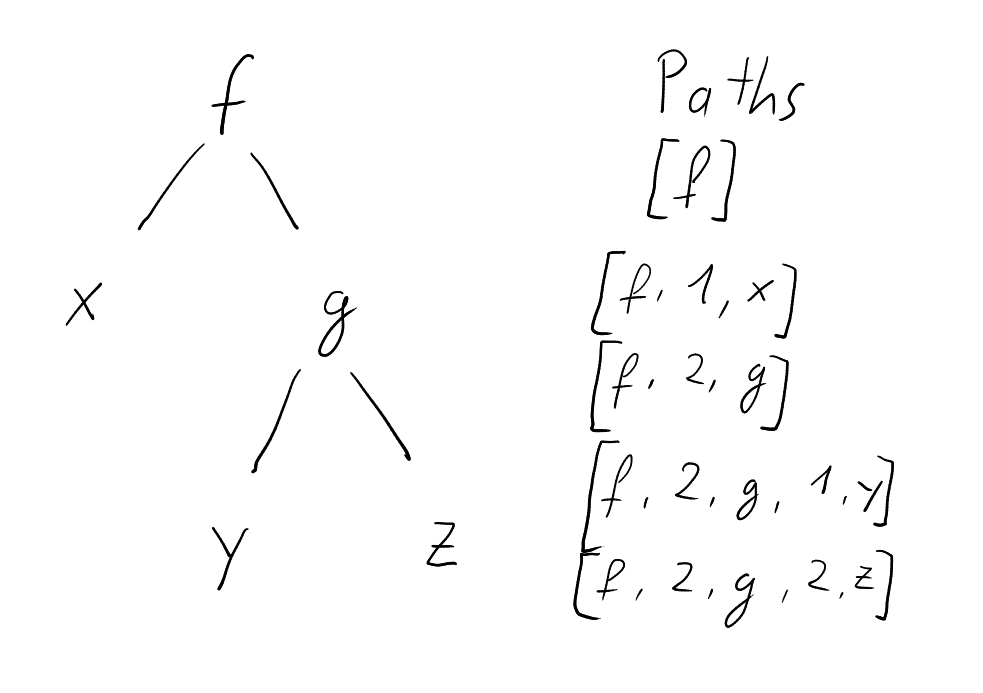
\includegraphics[scale=0.25]{figures/term_path.png}
\caption{A term and the paths associated with its symbols}
\end{figure}\todo{Path addresses a node, does not contain the last symbol}

To store the paths of different terms within one index we must associate each path with a list of terms which contain this path. We called these lists path lists. As a term is described by a path for each symbol each term is generally saved in many path lists.

For storage of the path lists we chose a trie-based approach. The index consists of nodes which each store two tables. The first table stores the path lists indexed by the last symbol in the path. The other table stores the children nodes index by a pair of symbols and indices. When we insert a path we start at the root and traverse the trie according to alternating sequence of the path. Once we reach the last symbol of the path we insert the path into the path list at that node. Inserting a term similar to one already present profits from the sharing of prefixes. This reduces the memory required as the paths of a term often share prefixes. An alternative approach is to store the path lists in a hash table.

The queries are based on intersections and unions of the different path lists to enforce constraints on the terms. The simplest query is the lookup of identical terms, for example to check if a term is already contained within the index. To answer the query we first build a list of the paths the term contains. Next we lookup the path lists corresponding to them in the index. The intersection of these path lists returns all terms containing symbols at identical paths as the query term. Under the assumption of consistent typing we retrieve only the original or no term as $f(x,y)$ can not exist simultaneously to $f(x)$.

To retrieve the unifiables of a term from the index we can use some observations regarding the unification problem.
\begin{enumerate}
  \item A variable is unifiable with any other term
  \item Every other symbol\todo{Name for ``every other symbol/terminal''? Fixed vars? Constants?} is unifiable with itself and variables
  \item A function $f(x_{1},...,x_{n})$ is unifiable with term $t$ if $t$ is a variable or the function symbols of $f$ and $t$ are identical and $x_{1},...,x_{n}$ are unifiable with the respective argument of $t$
\end{enumerate}
Using this we can define an algorithm recursing on the structure of the query term while intersecting and unifying the different path lists of the index. The different query types share parts with the lookup being the most restrictive and the unifiables the least restrictive.

We use the syntax $p \cdot f \cdot n$ to describe the path $p$ extended by the nth argument of the function $f$. $PathList(p)$ refers to the path list stored at the path $p$. $AllTerms$ is the collection of all terms stored in the index.
\begin{figure}[h]
\centering
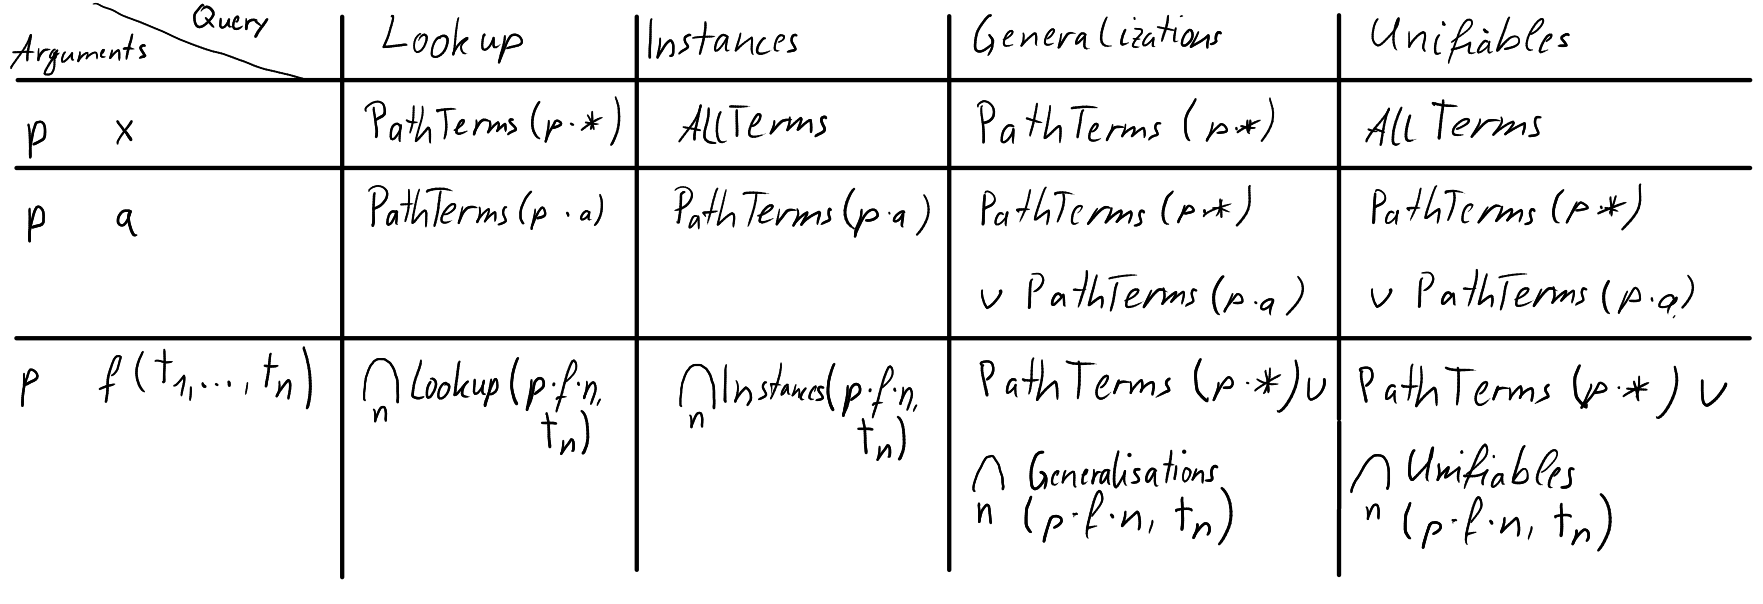
\includegraphics[scale=0.25]{figures/queries.png}
\caption{The different queries and their definition}
\end{figure}\\
We can see in the table that the different queries share many similarities with the $Unifiables$ being a combination of $Instances$ and $Generalizations$.

\section{Implementation in Isabelle/ML}
The efficient implementation of path indexing relies on a number of optimizations. The most common and performance critical operations are the queries which in turn rely on the union and intersection of the path lists. Unfortunately the interface of the already existing discrimination net allows the storage of arbitrary values addressed by terms. While this is unproblematic for discrimination nets it complicates path indexing.

First of all, the values stored in the path lists must be comparable to define set operations on them. Secondly, the comparison must also be extremely fast. While Poly/ML, the compiler on which Isabelle/ML is built, provides a pointer equality function, which is defined for any type, it does not guarantee equality for identical immutable values. Storing the values in mutable ref cells is also not an option as the Poly/ML runtime has significant overhead associated with them, both in memory consumption and garbage collection time.

Therefore we were presented with two options. Either we require the values to be comparable or we store an identifier together with every value at insertion where we still have the context to determine which paths belong to a value. The first approach prevents the path index from being used as a drop-in replacement for discrimination nets and complicates the usage, especially regarding an efficient comparison on complex data types. The second approach requires some additional memory to store the identifiers but offers multiple benefits. The user need not specify a comparison function or worry about its performance. We can rely on integer equality which is naturally extremely fast and need not use the pointer equality provided by Poly/ML which is reliant on runtime details like the merging of identical immutable values. This is quite important as we do not have any guarantee when the last heap compression occurred and manual invocation by using the ``shareCommonData'' introduces significant overhead to insertion. Additionally, reliance on low-level functions like ``shareCommonData'' and ``pointereq'' should be avoided as there are may be significant changes across runtime versions.

Another advantage of integer identifiers is that they are ordered. This allows us to use the OrdList module of the SML standard library for path lists and further speeds up the set operations.

We can further speed up the set operations by building a tree of the intersections and unions and only evaluating it at the end. This takes better advantage of the cache because the previously calculated list is not evicted from the cache by the trie traversal. Furthermore this presumably enables further compiler optimizations as the intermediate results are only short-lived and functions can be inlined.

Generic values.
Data Sharing in Poly/ML. Intersect at end for cache. Efficient intersect with OrdList. pointereq. Saving values separately. NoConstraint exc. No generic hash
